% Created 2023-02-23 Thu 18:44
% Intended LaTeX compiler: pdflatex
\documentclass{report}
                              \usepackage[utf8]{inputenc}
\usepackage[T1]{fontenc}
\usepackage{RJournal}
\usepackage{amsmath,amssymb,array}
\usepackage{booktabs}
\sectionhead{Contributed research article}
\volume{XX}
\volnumber{ZZ}
\year{20YY}
\month{MM}
\usepackage{blindtext}
\usepackage{xcolor}
\usepackage{listings}
\usepackage{hyperref}
\hypersetup{colorlinks=true, linkcolor=blue, filecolor=magenta, urlcolor=cyan}
\usepackage{float}
\DeclareMathOperator*{\argmax}{argmax}
\DeclareMathOperator*{\argmin}{argmin}
\newcommand{\J}{\ensuremath{J}}
\newcommand{\1}{\ensuremath{\mathbf{1}}}
\newcommand{\h}{\ensuremath{\lambda}}
\newcommand{\indep}{\ensuremath{\perp\hspace*{-1.4ex}\perp}}
\newcommand{\T}{\ensuremath{\widetilde{T}}}
\newcommand{\X}{\ensuremath{{W}}}
\renewcommand{\t}{\ensuremath{\Tilde{t}}}
\newcommand{\ax}{\ensuremath{\mid a,\,{w}}}
\newcommand{\aX}{\ensuremath{\mid A = a,\,{W}}}
\newcommand{\AX}{\ensuremath{\mid A,\,{W}}}
\newcommand{\x}{\ensuremath{{w}}}
\newcommand{\trt}{\ensuremath{\pi^*}}
\newcommand{\tk}{\ensuremath{t_{k}}}
\newcommand{\lj}{\ensuremath{l}}
\newcommand{\jj}{\ensuremath{j}}
\newcommand{\tK}{\ensuremath{K}}
\newcommand{\tKi}{\ensuremath{k}}
\newcommand{\TK}{\ensuremath{\mathcal{T}}}
\newcommand{\g}{\ensuremath{\pi}}
\renewcommand{\L}{\ensuremath{W}}
\renewcommand{\l}{\ensuremath{w}}
\newcommand{\tDelta}{\ensuremath{\widetilde{\Delta}}}
\newcommand{\F}{\ensuremath{\mathcal{F}}}
\setcounter{secnumdepth}{5}

\lstset{
keywordstyle=\color{blue},
commentstyle=\color{red},stringstyle=\color[rgb]{0,.5,0},
literate={~}{$\sim$}{1},
basicstyle=\ttfamily\small,
columns=fullflexible,
breaklines=true,
breakatwhitespace=false,
numbers=left,
numberstyle=\ttfamily\tiny\color{gray},
stepnumber=1,
numbersep=10pt,
backgroundcolor=\color{white},
tabsize=4,
keepspaces=true,
showspaces=false,
showstringspaces=false,
xleftmargin=.23in,
frame=single,
basewidth={0.5em,0.4em},
}
\renewcommand*\familydefault{\sfdefault}
\itemsep2pt
\author{imbroglio}
\date{\today}
\title{}
\begin{document}

\title{concrete R Paper: Title TBD}
\subtitle{}
\author{by David Chen, Thomas Gerds, Helene Rytgaard, Maya L. Petersen, Mark van der Laan, ...}

\maketitle

\abstract{
Competing risks are a common but under-addressed feature in biomedical survival studies. This article outlines a causal inference workflow that illuminates whether or not the researchers' question of interest involves competing risks and introduces the R package \CRANpkg{concrete} which implements a targeted maximum likelihood estimator for the cause-specific absolute risks for time-to-event outcomes measured in continuous or near-continuous time. The package can be used for survival analyses with or without competing risks and allows users to estimate causally-interpretable estimands such as risk ratios and risk differences using possibly misspecified cause-specific Cox models. Point estimates can be produced using G-formula plug-in or TMLE, and influence curve-based asymptotic inference will be provided for TMLE. Influence curve-based simultaneous inference is also possible if multiple times or events are targeted. This paper will demonstrate the use of \CRANpkg{concrete} using the PBC dataset.
}

Recently targeted maximum likelihood-based estimation (TMLE) has been used to develop estimators for cause-specific absolute risks of time-to-event outcomes measured in continuous time. \CRANpkg{concrete} implements in R a continuous-time TMLE for cause-specific absolute risks under static and dynamic interventions on a point treatment. \CRANpkg{concrete} can also return estimates and asymptotic inference for contrastive parameters such as risk differences and risk ratios. Risk estimands can be jointly targeted at multiple times, and in the case of competing risks, multiple cause-specific risks can be jointly targeted. In this paper we review the TMLE methodology implemented in \CRANpkg{concrete} and demonstrate its use and its features.

\section{Introduction}
\label{intro}
In many biomedical survival applications, study subjects are susceptible to competing risks. Recognizing this, authors have cautioned against the use of the standard survival estimands (\cite{andersen_competing_2012}, \cite{koller_competing_2012}, \cite{austin_accounting_2017}) and several methods have been developed for analyzing competing risks, including Fine-Gray regression (\cite{fine_proportional_1999}), pseudovalue regression (\cite{klein_regression_2005}), and direct binomial regression (\cite{scheike_predicting_2008}, \cite{gerds_absolute_2012}). Nevertheless, reviews of clinical literature by \cite{koller_competing_2012} and \cite{austin_accounting_2017} found that most published trials failed to adequately address the effect of potential competing risks in their studies. We suggest that this pattern results not from a lack of awareness, but rather from understandable confusion about when and how to choose an appropriate competing risks method. The remedy we propose is a causal roadmap (\cite{petersen_causal_2014}), guiding the process of 1) transforming a clinical question into a rigorously defined causal estimand, 2) translating that causal quantity into a statistical estimand while clearly addressing the necessary assumptions for doing so, and 3) estimating the target statistical quantity via a fully prespecified analysis that provides reliable inference and achieves desirable statistical properties such as efficiency and consistency. In Section \ref{concepts} we demonstrate a survival competing risks analysis following this roadmap and show how careful causal reasoning can clarify the process of making desirable statistical choices.



\CRANpkg{concrete} is an R package written to help researchers answer causal questions about the effect of interventions on time-to-event outcomes measured in continous time. Therefore, the package references concepts from causal inference even though \CRANpkg{concrete} can be used purely for statistical inference without causal ramifications. When we analyze data to guide future actions, we are in essence asking causal questions - questions that can be made rigorous with the formal frameworks developed in recent decades (\cite{pearl_causal_2016}, \cite{holland_statistics_1986}). Unfortunately the transition from causal thinking to statistical estimation is not always straightforward, and so a cohesive causal inference workflow ideally follows a structured roadmap (\cite{petersen_causal_2014}) that begins with 1) the causal model and causal estimands, 2) moves through identification to a statistical model and estimands, and then finally 3) performs estimation and provides inference. In subsequent sections we will briefly discuss these first two stages as they pertain to analyses of time-to-event data, but the majority of this manuscript will focus on the statistical estimation methodology implemented in \CRANpkg{concrete}. Rigorous and detailed discussions of these first two stages can be found elsewhere (\cite{laan_targeted_2011}, \cite{laan_targeted_2018}, \cite{rytgaard_continuous-time_2021}).

\subsection{What is in this manuscript}
\label{sec:orga384eb6}
We write for readers looking for a hands-on introduction to the one-step targeted maximum likelihood estimation (TMLE) method for continuous time survival analysis described in \cite{rytgaard_one-step_2021}, as well as for readers
wishing to use \CRANpkg{concrete} for their own analyses. In Section \ref{concepts} we briefly overview the one-step TMLE method as it is implemented in \CRANpkg{concrete} and in Section \ref{UsingConcrete} we demonstrate a competing risks analysis using \CRANpkg{concrete}. For a full and rigorous treatment of the one-step TMLE for continuous-time survival and competing risks, see \cite{rytgaard_one-step_2021} and \cite{rytgaard_continuous-time_2021}.

\subsection{What can concrete be used for}
\label{sec:orgeb349fd}
\CRANpkg{concrete} can be used for estimands derived from cause-specific absolute risks (e.g. risk ratios and risk differences) under static and dynamic interventions on binary treatments given at baseline. The currently implemented estimators are the one-step TMLE and a g-formula plug-in, and both can be applied to data involving baseline covariate confounding, right-censoring and competing risks. 

\CRANpkg{concrete} cannot yet investigate stochastic interventions or interventions on multinomial and continuous treatments. Currently only Cox models can be used for initial estimation of conditional hazards though the incorporation of penalized Cox (coxnet) and hazard estimators based on highly adaptive lasso (HAL) are planned in a future package version. Methods have not yet been implemented to account for time-dependent treatments (e.g. drop-in) or time-dependent confounding.

\CRANpkg{concrete} is not meant to be used for left trunctation (i.e. delayed entry), interval censored data, or clustered data; and it cannot assess the assumptions needed for causal identification. 

\subsection{How concrete relates to other peoples work}
\label{sec:orgfcc282a}
\CRANpkg{concrete} is the first general use R package implementing TMLE for continuous-time survival, with \href{https://github.com/helenecharlotte/continuousTMLE}{continuousTMLE} being the methods development package accompanying (\cite{rytgaard_one-step_2021}, \cite{rytgaard_continuous-time_2021}). The \CRANpkg{ltmle} (\cite{schwab_ltmle_2020}), \CRANpkg{stremr} (\cite{sofrygin_stremr_2017}), and \CRANpkg{survtmle} (\cite{benkeser_survtmle_2019}) packages either natively or can be adapted to perform discrete-time TMLE for absolute risks of right-censored survival outcomes; \CRANpkg{ltmle} and \CRANpkg{stremr} use the method of iterated expectations while \CRANpkg{survtmle} can target the hazard-based survival formulation. Notably these packages all implement discrete-time TMLEs and would necessitate discretizing continuous-time data which can negatively impact estimator performance. 

The \ctv{Causal Inference} CRAN Task View shows just \CRANpkg{riskregression} (\cite{gerds_riskregression_2022}) as expressly estimating treatment effect estimands in survival settings. \CRANpkg{riskregression} implements the g-formula plug-in, IPTW, and double-robust AIPTW estimators. The \ctv{Survival} CRAN Task View shows no packages to be implementing efficient semi-parametric estimators for survival estimands, though the non-CRAN  packages \href{https://github.com/RobinDenz1/adjustedCurves}{adjustedCurves} (\cite{denz_comparison_2022}) and \href{https://github.com/tedwestling/CFsurvival}{CFsurvival} (\cite{westling_inference_2021}) implement the AIPTW and a cross-fitted doubly-robust estimator respectively. 

\subsection{What concrete does}
\label{sec:org89ec992}
\CRANpkg{concrete} implements the one-step TMLE developed in \cite{rytgaard_one-step_2021} to estimate cause-specific absolute risks for interventions on point treatments and covariate measured at basleine. Asymptotic inference for TMLE estimates are derived from the variance of the efficient influence curve (EIC) (\cite{laan_unified_2003-1}). \CRANpkg{concrete} can also output estimates of risk differences and risk ratios, computed from absolute risk estimates with inference derived using the delta method.

Broadly speaking, this one-step TMLE procedure consists of two stages: 1) an initial estimation of nuisance parameters and 2) a targeted update of the initial estimators to solve the EIC of the target statistical estimand (\cite{laan_unified_2003-1}, \cite{kennedy_semiparametric_2016}).

For TMLE to be consistent and efficient, the initial nuisance parameter estimators must achieve certain convergence requirements. Unfortunately it is often impossible to know in advance which estimator is best suited for a particular estimation problem, and so in \CRANpkg{concrete} nuisance parameters are estimated using Super Learning, a cross-validated machine learning ensemble algorithm with oracle guarantees (\cite{laan_super_2007}, \cite{polley_superlearner_2021}, \cite{laan_unified_2003}, \cite{vaart_oracle_2006}). Super Learners with robust candidate libraries and valid loss functions give users the best chance of achieving the necessary conditions for TMLE's asymptotic properties. Guidance on how to best specify Superlearner estimators are discussed further in \cite{phillips_practical_2022}. Whenever possible, Super Learner libraries should include the highly adaptive lasso (HAL) which achieves the needed convergence rate (\cite{laan_generally_2017,benkeser_highly_2016,rytgaard_continuous-time_2021}) for TMLE's asymptotic properties.

The subsequent targeted update is based in semi-parametric efficiency theory (\cite{laan_targeted_2011}, \cite{kennedy_semiparametric_2016}), specifically that a regular, asymptotically linear estimator of a statistical estimand is efficient if its influence function is equal to the target estimand's EIC. By updating initial estimators of nuisance parameters to solve the EIC, TMLE can use flexible machine-learning algorithms for initial estimation, and still recover asymptotically valide inference. Contrary to other semi-parametric efficient estimators based on the influence function, TMLE is a plug-in estimator 

\subsection{concrete in a nutshell - PBC example}
\label{sec:org68daf60}
\lstset{language=r,label=pbc nutshell,caption= ,captionpos=b,numbers=none,otherkeywords={}, deletekeywords={}}
\begin{lstlisting}
# Prepare Data
library(concrete)
library(data.table)
library(tidyverse)
set.seed(12345)
data <- as.data.table(survival::pbc)
data <- data[!is.na(trt), ][, trt := trt - 1]
data <- data[, c("time", "status", "trt", "age", "sex", "albumin")]

# Specify Analysis
ConcreteArgs <- formatArguments(DataTable = data,
				EventTime = "time",
				EventType = "status",
				Treatment = "trt",
				Intervention = makeITT(),
				TargetTime = 90 * (6:30),
				TargetEvent = 1:2,
				MaxUpdateIter = 500)
# Compute
ConcreteEst <- doConcrete(ConcreteArgs)

# Return Output
ConcreteOut <- getOutput(ConcreteEst, Estimand = "RD")
plot(ConcreteOut, Estimand = "RD", GComp = TRUE, ask = FALSE)
\end{lstlisting}

\begin{figure}[H]
\center
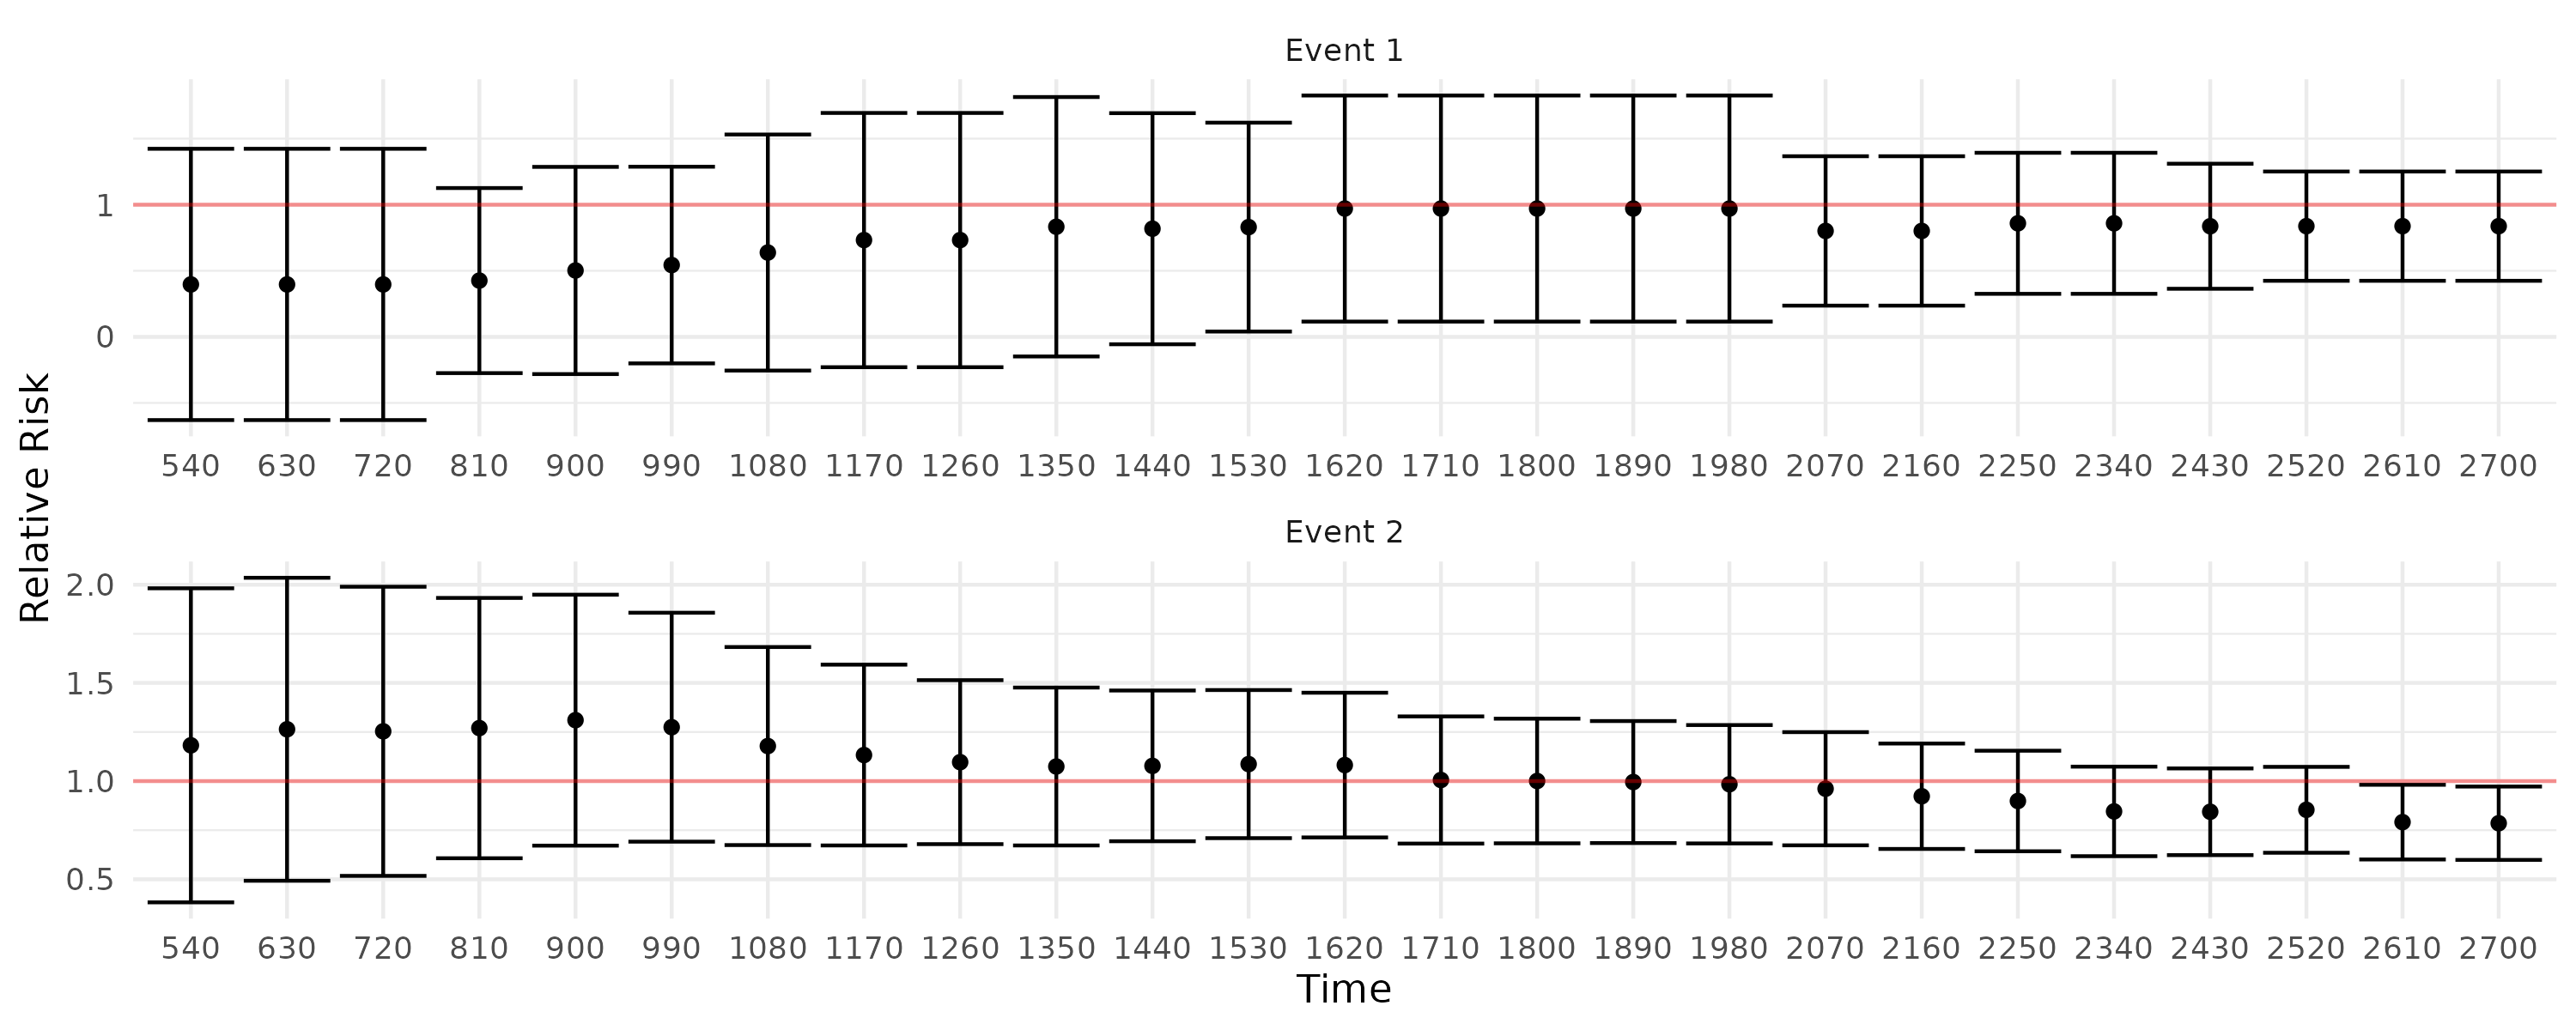
\includegraphics[width=\linewidth]{fig/RR.png}
\end{figure}

\section{Concepts}
\label{concepts}
\subsection{The Targeted Learning Roadmap}
\label{sec:orgc11b1ac}
A basic targeted learning roadmap for analyzing continuous-time survival or competing risks consists of:
\begin{enumerate}
  \item Defining the causal model and specifying a causal estimand (e.g. causal risk difference at time $t$). Considerations include defining time zero and a time horizon, identifying the intervention (i.e. treatment) variable, specifying the desired intervention(s), specifying the event(s) of interest.
  \item Defining the statistical model and the statistical estimand, while stating and discussing the assumptions necessary for the statistical estimand to identify the causal estimand. Considerations include identifying confounding variables and sources of right-censoring, establishing positivity for censoring and desired interventions, and formalizing knowledge about the statistical model (e.g. dependency structures or functional structures such as proportional hazards).
  \item Performing estimation and providing inference. Considerations include choosing an estimator with desirable properties (e.g. consistency and efficiency within a desired class), using outcome-blind simulations to practically assess the estimator's robustness and usability, and pre-specifying the estimation procedure to avoid misleading inference.
\end{enumerate}

In the following sections we discuss the steps in this roadmap in more detail.

\subsection{The Causal Model: Counterfactuals, Interventions, and Causal Estimands}
\label{sec:org9f45dd3}
With time-to-event data, the counterfactual outcomes are how long it takes for some event(s) occur if subjects hypothetically receive some intervention. Let \(A\) be this intervention variable and let \(d\) be the intervention rule, i.e. the function that assigns values to \(A\). The simplest interventions are static rules to set \(A\) to some value \(a\), \(d = a\). More flexible dynamic treatment rules might assign treatments based on subjects' baseline covariates, while stochastic treatment rules incorporate randomness may even depend on the natural treatment assignment mechanism. Whatever the desired intervention, let \(d\) represent the intervention of interest and let \(\L\) represent subjects' baseline covariates. Then a counterfactual survival dataset with \(J\) competing events, an intervention \(d\) delivered at baseline (i.e. time zero), and a time horizon of \(t_{max}\) takes the form:
\begin{equation}
 X = \left(T^d,\, \Delta^d,\, \L \right) \label{causaldata}
\end{equation}
where \(T^d \in (0, t_{max}]\) is earliest occurence of any of the \(J\) events under intervention \(d\), and \(\Delta^d \in \{1, \dots, J\}\) shows which of the \(J\) events occured first under intervention \(d\). Notably, we do not include censoring in this counterfactual data and instead isolate just those events that experimenters would want to observe in their ideal hypothetical experiment. For ideal experiments tracking just one event, the causal setting is one of classic survival; if instead mutually exclusive events would be allowed to compete, then the causal setting is one with competing risks. 

With the counterfactual data defined, causal estimands can then be specified as functions of this data. For instance, the causal event-\(\jj\) relative risks under some interventions \(d^*\) versus \(d^{**}\) can be written as Eq. \eqref{causalrisk} 

\begin{equation}
\Psi^\F_{F_{j,t}} = P(T^{d^*} \leq t, \Delta^{d^*} = j) / P(T^{d^{**}} \leq t, \Delta^{d^{**}} = j) \label{causalrisk}
\end{equation}
and the causal difference in event-free survival at time \(t\) as Eq. \eqref{causalsurv}.
\begin{equation}
\Psi^\F_{S_t} = P(T^{d^*} < t) - P(T^{d^{**}} < t) \label{causalsurv}
\end{equation}

Researchers may be interested in these estimands at a single endpoint or at many timepoints, potentially even full risk curves over a time interval (e.g. \(\Psi^\F_{F_{j,t}} : t \in (0, t_{max}]\)). In the case of competing risks, researchers may also be simultaneously interested in multiple cause-specific estimands (e.g. \(\Psi^\F_{F_{j,t}} : j \in 1, \dots, J\)). These estimands, and others, can all be rigorously defined as functions of the counterfactual data; efforts can then be made in the next step to identify these causal estimands with functions of observed data, i.e. statistical estimands.

\subsection{Observed Data, Identification, and Statistical Estimands}
\label{ObservedData}
Observed time-to-event data with \(J\) competing events might be written as:
\begin{equation}
 O = \left(\T,\, \tDelta,\, A,\, \L \right) \label{obs-data}
\end{equation}
where \(\T \in (0, t_{max}]\) is the earlier of the first event time \(T\) or the right-censoring time \(C\), \(\tDelta \in \{0, \dots, J\}\) indicates which event occurs (with 0 indicating right-censoring), \(A\) is the observed treatment and \(\L\) is the set of baseline covariates.

To link causal estimands such as Eq. \eqref{causalrisk} and \eqref{causalsurv} to statistical estimands, we then need several untestable identification assumptions to hold: consistency, positivity, no unmeasured confounding, and conditionally independent censoring (For more details, see Section 3 in \cite{rytgaard_continuous-time_2021}). Given these assumptions, the cause-\(j\) absolute risk at time \(t\) under intervention \(d\) can be identified by the g-computation formula
\begin{align}
F^d_j(t) &= \mathbb{E}_{\mathcal{\L}} \left[ \mathbb{E}_{\g^d} \left[{ F_j(t \ax)} \right] \right] \nonumber \\
&= \mathbb{E}_{\mathcal{\L}} \left[ \int_{\mathcal{A}} \,  \left[{ \int_0^t \lambda_j(s \ax) \, S(s- \ax) \, ds }\right] \, \g^d (a \mid \l) \, da \right] \label{absrisk}
\end{align}
where the cause-\(j\) conditional hazard at time \(t\) is
\begin{equation*}
\lambda_j(t \ax) = \lim\limits_{h \to 0} \frac{1}{h} P(\T \leq t + h,\, \tDelta = j \mid \T \geq t,\, a,\, \x) 
\end{equation*}
the conditional event-free survival at time \(t\) is 
\begin{equation*}
S(t \ax) = \exp\left(-\int^{t}_{0} \sum\limits_{j=1}^{J} \lambda_j(s \ax) \, ds \right)
\end{equation*}
and \(\g^d(a \mid \l)\) is the treatment propensity implied by the intervention \(d\).

With this identification result in Eq \eqref{absrisk}, the causal cause-\(j\) relative risk \eqref{causalrisk} is simply identified by the statistical estimand \eqref{obsrisk} 
\begin{equation}
\Psi_{F_{j,t}} = F^{d^*}_j(t) \;\; / \;\; F^{d^{**}}_j(t) \label{obsrisk}
\end{equation}
and the causal difference in survival \eqref{causalsurv} estimand can then be identified by the statistical estimand \eqref{obssurv}.
\begin{equation}
\Psi_{S_{t}} = \left[1 - \sum_{j = 1}^{J} \, F^{d^*}_j(t) \right] - \left[1 - \sum_{j = 1}^{J} \,  F^{d^{**}}_j(t) \right] \label{obssurv}
\end{equation}

It should be noted here that when the identification assumptions do not hold, these statistical estimands in Eq. \eqref{obsrisk} and \eqref{obssurv} may still have valuable interpretations as standardized risks isolating the importance of the "intervention" variable (\cite{laan_statistical_2006}).

\subsection{Targeted Estimation}
\label{estimation}
The TMLE procedure for estimands derived from cause-specific absolute risks begins with estimating the treatment propensity \(\g\), the conditional hazard of censoring \(\lambda_c\) and the conditional hazards of events \(\lambda_j \,:\; j = 1, \dots, J\). In \CRANpkg{concrete} these nuisance parameters are estimated using the Super Learner algorithm, which involves specifying a cross-validation scheme, compiling a library of candidate algorithms, and designating a cross-validation loss function and a Super Learner meta-learner.

\subsubsection{Specifying Super Learners}
\label{cv}
For \(V\text{-fold}\) cross validation, let \(Q_n = \{O_i\}_{i=1}^n\) be the observed \(n\) i.i.d observations of \(O \sim P_0\) and let \(B_n = \{1, ... , V\}^n\) be a random vector that assigns the \(n\) observations into \(V\) validation folds. For each \(v \in \{1, ..., V\}\) we then define a training set \(Q^\mathcal{T}_v = \{O_i : B_n(i) = v\}\) with the corresponding validation set \(Q^\mathcal{V}_v = \{O_i : B_n(i) \neq v\}\). 

When specifying Super Learner libraries, candidate algorithms should range in flexibility and while respeciting pre-existing knowledge about the data-generating mechanism should be selected. For instance, candidate estimators for conditional hazards should incorporate domain knowledge about which covariates may be most predictive of event times. If the number of independent observations \(n\) is much greater than the number of covariates, then more highly flexible candidate algorithms such as Highly Adaptive Lasso (HAL) should be included in the Super Learner library. If on the other hand the number of covariates is not much less than \(n\), then libraries should be comprised of fewer and less flexible candidate algorithms,  potentially with native penalization as with coxnet or being paired with covariate screening algorithms.

Super Learner loss functions should be bounded and minimized by the true data-generating process and for maximal robustness, the discrete selector that simply selects the best performing candidate should be used as the Super Learner metalearner.

Currently the default cross-validation setup in \CRANpkg{concrete} attempts to follow the guidelines laid out in \cite{phillips_practical_2022}, with the number of cross-validation folds increasing as sample size decreases. Default Super Learner libraries are provided, but should be amended to suit users' data as detailed above. Further details on the default \CRANpkg{concrete} Super Learner specifications for each nuisance parameter are provided in the following sections.

\subsubsection{Estimating Treatment Propensity}
\label{trtps-est}
For estimating the treatment propensity, let \(\g_0(\cdot \mid \X)\) be the true conditional distribution of \(A\) given \(\X\), \(\mathcal{M}_{\g} = \left\{\Hat{\g} : Q_n \to \Hat{\g}(Q_n) \right\}\) be the candidate library of propensity score estimators, and \(L_\g\) be a loss function such that the risk \(\mathbb{E}_0\left[L_\g(\Hat{\g}, O)\right]\) is minimized when \(\Hat{\g} = \g_0\). The current \CRANpkg{concrete} default for estimating treatment propensity uses the default \CRANpkg{Superlearner} loss functions with glmnet and xgboost as candidate algorithms. The discrete Superlearner estimator is then the the candidate propensity estimator \(\Hat{\g} \in \mathcal{M}_{\g}\) that has minimal cross validated risk
\begin{equation}
\Hat{\g}^{SL} = \argmin_{\Hat{\g} \in \mathcal{M}_\g} \sum_{v = 1}^{V} P_{Q^\mathcal{V}_v} \; L_\g(\Hat{\g}(Q^\mathcal{T}_v), Q^\mathcal{V}_v) \label{propsl}
\end{equation}


\subsubsection{Estimating Conditional Hazards}
\label{haz-est}
For estimating the conditional hazards, let \(\lambda_{0,\,\delta} \,:\; \delta = 0, \dots, J\) be the true conditional hazards for censoring (\(\delta = 0\)) and events (\(\delta \in \{1, \dots, J\}\)). Let \(\mathcal{M}_\delta = \{\Hat{\lambda}_\delta : Q_n \to \mathbb{R}\}\) for \(\delta = 0, \dots, J\) be the libraries of candidate estimators for the censoring and cause-specific hazards. The current \CRANpkg{concrete} default is a library of two Cox models, treatment-only and main-terms. The corresponding loss function is then the negative log Cox partial-likelihood loss function \(L_\delta(\beta) = - \sum_{i=1}^{n} \left[\beta\,\L_i - \log\left[\sum_{h \in \mathcal{R}(\T_h)} \exp(\beta\,\L_h)\right]\right] \,\). The discrete SuperLearner selector for each \(\delta\) chooses the candidate \(\Hat{\lambda}_\delta \in \mathcal{M}_\delta\) that has minimal cross validated risk 
\begin{equation}
\Hat{\lambda}_\delta^{SL} = \argmin_{\Hat{\lambda}_\delta \in \mathcal{M}_\delta} \sum_{v = 1}^{V} P_{Q^\mathcal{V}_v} \; L_\g(\Hat{\lambda}_\delta(Q^\mathcal{T}_v), Q^\mathcal{V}_v) \;:\; \delta = 0, \dots, J\label{hazsl}
\end{equation}

These conditional hazard estimators are then used to compute the cause-specific absolute risks and survivals that are needed to compute the efficient influence curve (EIC). 

\subsubsection{Solving the Efficient Influence Curve}
\label{EIC}
The treatment propensity estimator Eq. \eqref{propsl} and conditional hazard estimators Eq. \eqref{hazsl} are used to compute the cause-specific absolute risk EICs corresponding to estimands like Eq. \eqref{obsrisk} and \eqref{obssurv}. Parameters that contrast multiple cause-specific absolute risks at multiple time points involve vector EICs comprised of the absolute risk EICs for each targeted event, each target time, and each intervention. For example, the vector EIC element corresponding to the event \(\jj\), time \(t\), and intervention propensity \(\trt\) cause-specific absolute risk (\(\Psi_{\trt, \jj, t}(P_0) = F_\jj^{\trt}(t)\)) is:
\begin{align}
    D^*_{\trt, \jj, t}(\lambda, \g, S_c)(O) = \sum_{\lj = 1}^{J} \int \; &h_{\trt,\, \jj,\, \lj,\, t, s}(\lambda, \g, S_c)(O) \, \left(N_{\lj}(ds) - \1(\T \geq s) \, \lambda_\lj(s \AX)\right) \label{eic} \\
    &{\color{blue!60!black}+ \sum_{a\,\in\,\mathcal{A}} F_\jj(t \mid A = a, \X)\,\trt(a \mid \X) - \Psi_{\trt, \jj, t}(P_0)}  \nonumber 
\end{align}
where \(N_l(s) = \1\left\{\T \leq s, \tDelta = l\right\}\) are the cause-specific counting processes and \(h_{\trt,\, \jj,\, \lj,\, t,\, s}(\lambda, \g, S_c)(O)\) is the TMLE "clever covariate" with the form
\begin{align}
    h_{\trt,\, \jj,\, \lj,\, t,\, s}&(\lambda, \g, S_c)(O) = \frac{{\color{blue}\trt(A \mid \X)\,} \1(s \leq t)}{{\color{green!70!black}\g(A \mid \X) \;S_c(s\text{-} \AX)}} \, \bigg(\1(\lj = \jj) - \frac{{\color{red}F_\jj(t \AX)} - {\color{red} F_\jj(s \AX)}}{{\color{red} S(s \AX)}}\bigg) \label{clevcov}
\end{align}
where \(F_j(t \ax)\) is the conditional cause-\(j\) absolute risk, \(S_c(t \AX)\) is the conditional censoring survival, \(S(t \AX)\) is the conditional event-free survival, and \(N_j(t) = \1\{\T \leq t, \, \Delta = l\}\) is the event-\(j\) counting process. The treatment propensity \(\g\) and the conditional event and censoring hazard functions ( \(\lambda_c,\, \lambda_j \;:\;  j = 1, \dots, J\)) are directly estimated with Eq. \eqref{propsl} and \eqref{hazsl} while the conditional absolute risks and survivals are computed from the hazard estimates as described in Section \ref{ObservedData}. The clever covariate is a function of the {\color{blue}intervention propensity}, {\color{green!70!black}observed conditional distributions} which are not changed by TMLE targeting, and lastly the {\color{red}outcome-related conditional distributions} which are updated by targeting.

The one-step continuous-time survival TMLE updates the cause-specific hazards along the universally least favorable submodel in the following manner:
\begin{equation}
\lambda_{j, \epsilon}(t) = \lambda_{j}(t) \, \exp\left(\int_{0}^{\epsilon}\frac{\left<\mathbb{P}_n \tilde{D}^*( \lambda_{x}, \g,  S_c)(O),\; h_{j, s}( \lambda_{x}, \g,  S_c)(O) \right>_{\Sigma}}{|| \tilde{D}^*( \lambda_{x}, \g, S_c)(O)||_{\Sigma}} \; dx \right) \label{onestep}
\end{equation}
where
\begin{align*}
\left<x , y \right>&_{\Sigma} = x^\top \Sigma^{\text{ -}1} y \hspace{.5cm}, \hspace{.5cm} ||x||_{\Sigma} = \sqrt{x^\top \Sigma^{\text{ -}1} x}
\intertext{\(\tilde{D}^*\) is the vector of efficient influence functions}
\tilde{D}^{*}(\lambda, \g, S_c)(O) &= \left(D^*_{\trt, \jj, \tk}(\lambda, \g, S_c)(O) : \trt \in \mathcal{A}, \jj \in \mathcal{J}, \tk \in \TK)\right)
\intertext{and \(h_{j, s}\) is the vector of clever covariates}
h_{j, s}(\lambda, \g, S_c)(O) &= \left(h_{\trt, \jj, \lj, \tk, s}(\lambda, \g, S_c)(O) : \trt \in \mathcal{A}, \jj \in \mathcal{J}, \tk \in \TK)\right)
\end{align*}

In practice this integral is approximated by recursively summing along a series of locally least favorable models and ends when 

\begin{equation}
\mathbb{P}_n D^*(\lambda_{\epsilon}, \g, S_c)(O) \leq \frac{\sqrt{\mathbb{P}_n \;D^*( \lambda_{\epsilon}, \g, S_c)(O)^2}}{\sqrt{n} \, \log(n)} \label{one-step-stop}
\end{equation}

\subsubsection{Estimating Variance}
\label{sec:org42ef92a}

In \CRANpkg{concrete}, the variance of TMLE estimates of targeted risks is computed by dividing the corresponding EIC's variance by the sample size, \(\frac{\mathbb{P}_n \;D^*( \lambda_{\epsilon}, \g, S_c)(O)^2}{n}\), which is a consistent estimator of the asymptotic variance of asymptotically linear estimators. In the presence of significant positivity violations (which may be seen as propensity scores close to 0), this EIC-derived variance estimator will be anti-conservative and variance estimation by bootstrap may be more reliable. However, bias resulting from positivity violations cannot be remedied in this way, and so other methods of addressing positivity violations (\cite{petersen_diagnosing_2012}) are recommended instead. For multidimensional estimands, simultaneous confidence intervals can be computed by simulating the \(1 - \alpha\) quantile of a multivariate normal distribution with the correlation structure of the estimand EICs.

\section{Usage}
\label{UsingConcrete}
There are 3 main user-facing functions in \CRANpkg{concrete}: \code{formatArguments()}, \code{doConcrete}, and \code{getOutput}. Specification of the estimation problem is done through input into \code{formatArguments()}, which checks the estimation specification and outputs a \code{"ConcreteArgs"} object that encapsulates the estimation specification. When the estimation procedure is adequately specified, the \code{"ConcreteArgs"} object then passed into \code{doConcrete()} to perform the specified continuous-time one-step survival TMLE. The output of \code{doConcrete()} is a \code{"ConcreteEst"} object which can be passed into getOutput to output tables and plots for cause-specific absolute risk derived estimands such as risk differences and relative risks. 

\subsection{formatArguments()}
\label{formatArguments}

\subsection{ConcreteArgs}
\label{sec:org709211d}
The arguments of \code{formatArguments()} are primarily involved in specifying 1) the observed data structure, 2) the target estimand, and 3) the TMLE estimator.

\lstset{language=r,label= ,caption= ,captionpos=b,numbers=none,otherkeywords={}, deletekeywords={}}
\begin{lstlisting}
data <- as.data.table(survival::pbc)
data <- data[, c("time", "status", "trt", "age", "sex", "albumin")]
data <- data[!is.na(trt), ][, trt := trt - 1]

ConcreteArgs <- formatArguments(DataTable = data,
				EventTime = "time",
				EventType = "status",
				Treatment = "trt",
				ID = NULL, 
				Intervention = 0:1,
				TargetEvent = 1:2,
				TargetTime = 90 * (6:30),
				MaxUpdateIter = 500)
\end{lstlisting}

\subsubsection{Data}
\label{ObservedDataConcrete}
Observed data is passed into the \code{DataTable} argument as either a \code{data.frame} or \code{data.table} object. This data must include columns corresponding to the observed times \(\T\), indicator of which event occured (\(\Delta\), and treatment variable \(A\), as well as any number of columns containing baseline covariates \(\L\). Note that the treatment values in \(A\) must be numeric, with binary treatments encoded as 0 or 1. The data must not have missingness; imputation of missing covariates should be done prior to passing data into \CRANpkg{concrete} while data with missing treatment or outcome values is not supported by \CRANpkg{concrete}. If the data includes a column with uniquely identifying subject IDs, its name should be passed into the \code{ID=} argument; this is for compatibility with planned future functionality for analyzing clustered or longitudinal data.

In the above PBC example, the observed data is contained in the \code{data} object, \(\T\) is the column \{"time"\}, \(\Delta\) is the column \{"status"\}, \(A\) is the column \{"trt"\}, and covariates \(L\) are the remaining columns: "age", "sex", and "albumin".

\subsubsection{Target Estimand}
\label{Estimand}
\CRANpkg{concrete} implements a continuous-time one-step TMLE targeting absolute risk derived estimands indexed by  interventions, target events, and target times.  

\paragraph{Intervention}
\label{TreatmentRegime}
For a binary \(A\) and static interventions \(d\) setting all observations to \(A=0\) or \(A=1\), interventions can specified with 0, 1, or c(0, 1) for both. More complex interventions can be specified with a list containing a pair of functions: an "intervention" function which outputs desired treatment \textbf{\textbf{assignments}} and a "g.star" function which outputs desired treatment \textbf{\textbf{probabilities}}. Dynamic interventions can be passed in as "intervention" functions without an accompanying "g.star" function, while stochastic interventions should be passed in as "g.star" functions. These functions can take treatment and covariates as arguments and must produce treatment assignments and probabilities respectively, each with the same dimensions as the observed treatment. The function \code{makeITT()} creates list of functions corresponding to binary static interventions, which can be used as a template for specifying more complex interventions.

\paragraph{Target Events}
\label{TargetEvent}
The \code{TargetEvent} argument specifies the event types of interest. Event types must be be coded as integers, with 0 reserved for censoring. If \code{TargetEvent=} is left \code{NULL}, then all non-zero event types present in the observed data will be targeted.

In the \code{pbc} dataset, there are 3 event values encoded by the \code{status} column: 0 for censored, 1 for transplant, and 2 for death. To analyze \code{pbc} with transplants treated as right-censoring, \code{TargetEvent} should be set to 2,
whereas for a competing risks analysis one could either leave \code{TargetEvent = NULL} or set \code{TargetEvent = 1:2} as in the above example.

\paragraph{Target Time}
\label{TargetTime}
The \code{TargetTime=} argument specifies the time(s) at which estimates of the cause-specific absolute risks or event-free survival are desired. Target times should be restricted to the time range in which target events are observed and \code{formatArguments()} will return an error if target time is after the last observed failure event time. If no \code{TargetTime} is provided, then \CRANpkg{concrete} will target the last observed event time, though this is likely to result in a highly variable estimate if prior censoring is substantial. The \code{TargetTime=} argument can either be a single number or a vector, as one-step TMLE can target cause-specific risks at multiple times simultaneously. For estimands involving full curves, \code{TargetTime=} should be set to a fine grid covering the desired interval.

\subsubsection{Estimator Specification}
\label{EstimationSpec}
The \code{formatArguments()} arguments involved in estimation are the cross-validation setup \code{CVArg}, the Superlearner candidate libraries \code{Model}, the software backends \code{PropScoreBackend} and \code{HazEstBackend}, and the practical TMLE implementation choices \code{MaxUpdateIter}, \code{OneStepEps}, and \code{MinNuisance}. Note that \code{Model} is used in this section in line with common usage in statistical software, rather than to refer to statistical or causal models as in preceding sections. 

\paragraph{Cross-Validation}
\label{CV}
\CRANpkg{concrete} uses \CRANpkg{origami} to specify cross-validation folds, specifically the function
\code{origami::make\_folds()}. If no input is provided to the \code{formatArguments(CVArg= )} argument, concrete will implement simple V-fold cross-validation following the recommendations in \cite{phillips_practical_2022}.

\lstset{language=r,label= ,caption= ,captionpos=b,numbers=none,otherkeywords={}, deletekeywords={}}
\begin{lstlisting}
CVArgs <- list(n = nrow(data), V = 10)
\end{lstlisting}

\paragraph{Estimating Nuisance Parameters}
\label{NuisanceEstimation}
Super Learner libraries for estimating nuisance parameters are specified in the \code{Model} argument. The input should be a named list with an element for the treatment variable and one for each event type including censoring. The list element corresponding to treatment must be named with the column name and the list elements corresponding to each event type must be named for the numeric value of the event type (e.g. "0" for censoring). Any missing specifications will be filled in with defaults, and the resulting list of libraries can be accessed in the output \code{.[["Model"]]} which can be then edited by the user.

\lstset{language=r,label= ,caption= ,captionpos=b,numbers=none,otherkeywords={}, deletekeywords={}}
\begin{lstlisting}
Model <- list("trt" = c("SL.glmnet", "SL.ranger", "SL.xgboost", "SL.glmn"),
	      "0" = list("~ trt", "~ ."),
	      "1" = list("~ trt", "~ .", "~ trt:.")
	      "2" = list("~ trt", "~ .", "~ trt:.")
	      )
\end{lstlisting}

\paragraph{Propensity Score}
\label{PropScore}
In \CRANpkg{concrete}, propensity scores are by default estimated using the \CRANpkg{SuperLearner}
package \code{formatArguments(PropScoreBackend = "Superlearner")} with candidate algorithms \code{c("xgboost", "glmnet")} implemented by packages \CRANpkg{xgboost} and \CRANpkg{glmnet}. Alternatively the \CRANpkg{sl3} package can be used by specifying \code{formatArguments(PropScoreBackend = "sl3")}.

\paragraph{Event and Censoring Hazards}
\label{HazardEstimation}
For estimating the necessary conditional hazards, \CRANpkg{concrete} currently relies on a discrete Superlearner consisting of a library of Cox models implemented by \code{survival::coxph()} evaluated on cross-validated pseuo-likelihood loss. Support for estimation of hazards using Poisson-HAL or other methods may be added in the future, but currently the \code{HazEstBackend} argument must be "coxph". The default Cox specifications are a treatment-only model and a main-terms model with treatment and all covariates. 

\paragraph{TMLE Specification}
\label{tmle-specification}
As detailed by Eq. \eqref{onestep} and \eqref{one-step-stop}, the one-step TMLE update step involves recursively updating cause-specific hazards, summing along small steps \(\epsilon_i\). 

The \code{formatArguments(MaxUpdateIter= )} argument is provided to provide a definite stop to the recursive TMLE update. The default number is 500 and should be sufficient for most applications, but may need to be increased when support for targeted estimands in the data is low and when targeting estimands with many components.

The argument \code{formatArguments(MinNuisance= )} can be used to specify a lower bound for the product of the propensity score and lagged survival probablity for remaining uncensored; this term is present in the denominator of the efficient influence function and enforcing a lower bound decreases estimator variance at the cost of introducing bias but improving stability.

\paragraph{ConcreteArgs object}
\label{concreteargs}
\code{formatArguments()} returns a list object of class \code{"ConcreteArgs"}. This object can be modified by the user and then passed back through \code{formatArguments()} in lieu of supplying new inputs directly into \code{formatArguments()}.

\lstset{language=r,label= ,caption= ,captionpos=b,numbers=none,otherkeywords={}, deletekeywords={}}
\begin{lstlisting}
  ConcreteArgs$Verbose <- TRUE
ConcreteArgs[["Model"]][["1"]][[3]] <- "~ trt:."
  ConcreteArgs <- formatArguments(ConcreteArgs)
\end{lstlisting}

The print method for ConcreteArgs objects displays summary information about 1) the observed data, 2) the target estimand (i.e. target event(s), target time(s) and intervention(s)), 3) specifications for initial nuisance parameter estimation, and 4) specification for the TMLE update. 

\lstset{language=r,label= ,caption= ,captionpos=b,numbers=none,otherkeywords={}, deletekeywords={}}
\begin{lstlisting}
print(ConcreteArgs, Verbose = FALSE)
\end{lstlisting}

\begin{figure}[H]
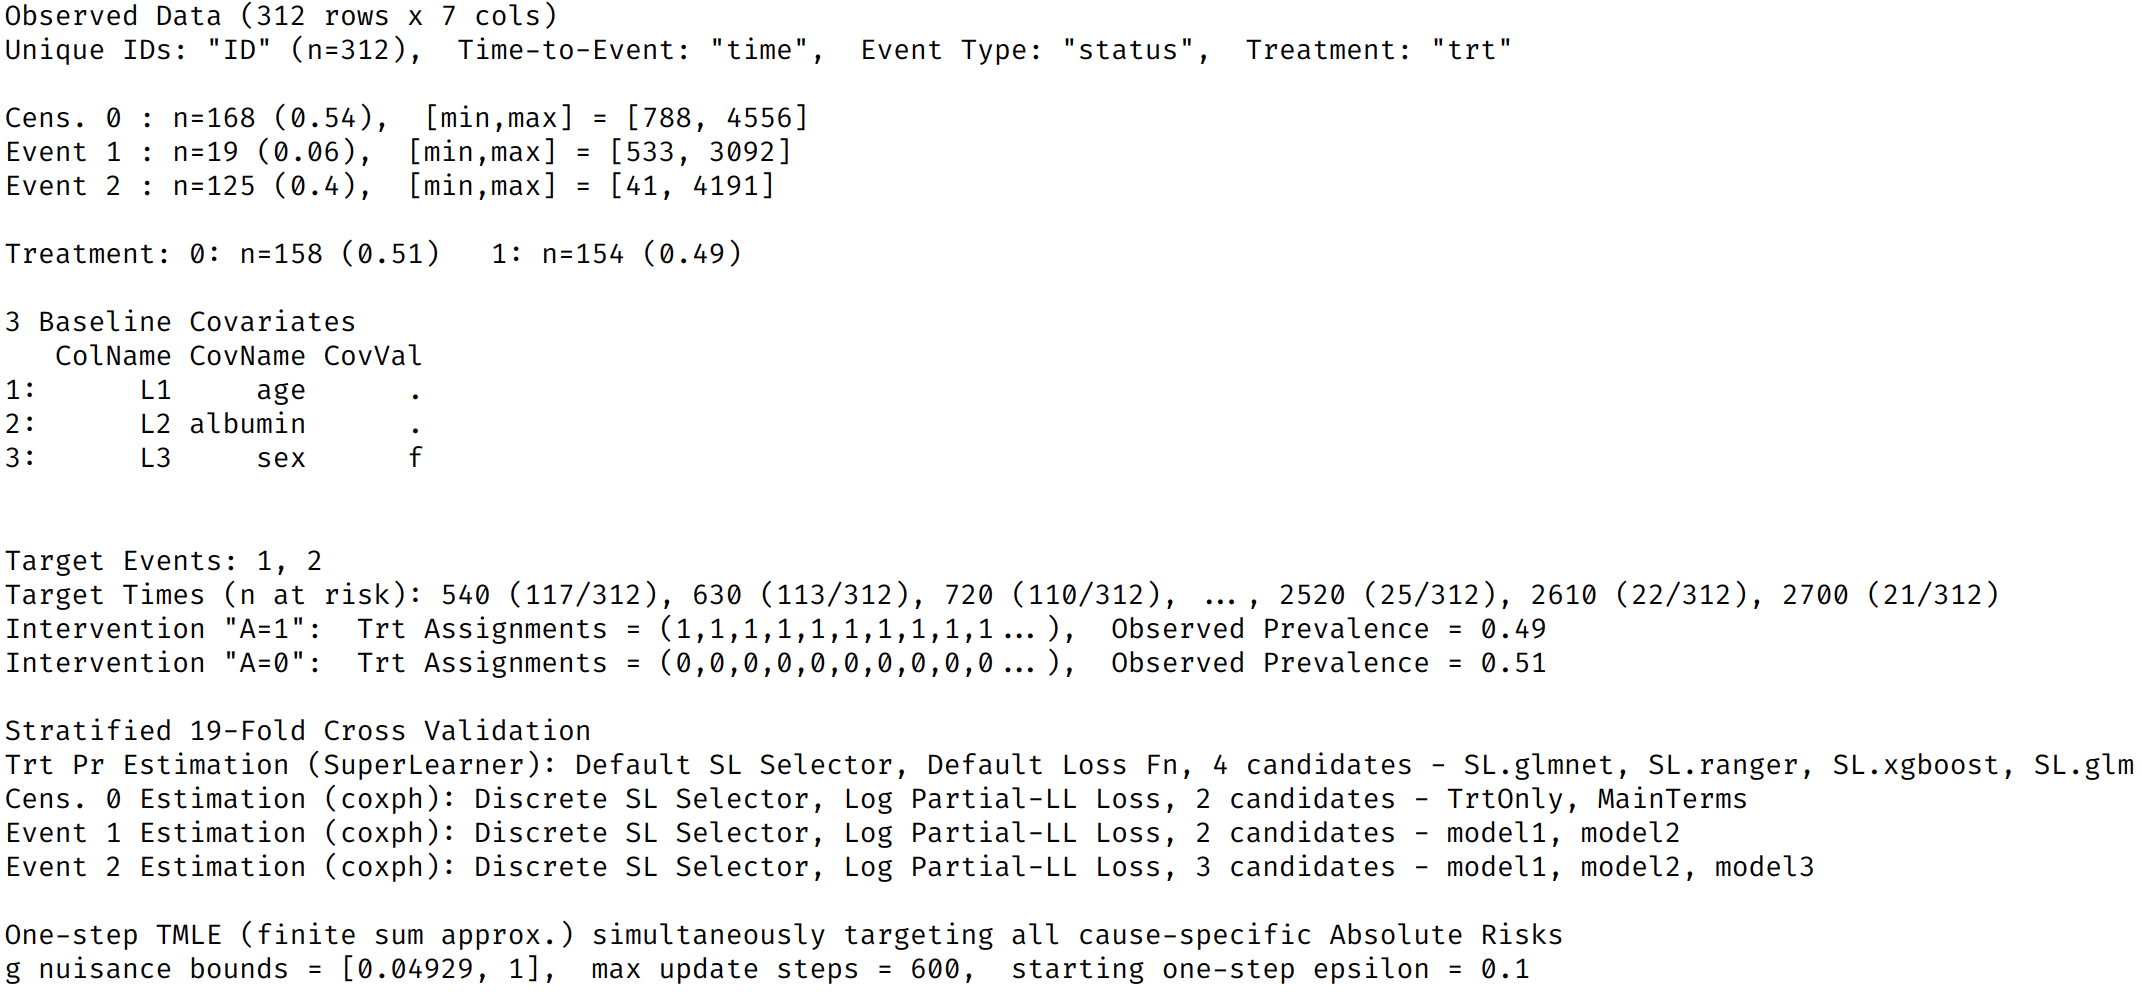
\includegraphics[width=\linewidth]{fig/ConcreteArgs.png}
\end{figure}

\subsection{doConcrete()}
\label{doConcrete}
Once \code{formatArguments()} runs satisfactorily, the resulting object of class \code{"ConcreteArgs"} is passed into the \code{doConcrete()} function which will then perform the specified TMLE algorithm. The output is an object of class \code{"ConcreteEst"} which contains TMLE point estimates and influence curves for the cause-specific absolute risks for each targeted event at each targeted time. If \code{formatArguments(GComp=TRUE)}, then the \code{"ConcreteEst"} object will also contain the result of using the Superlearner predictions as a plug-in g-formula estimate of the targeted risks. 

\lstset{language=r,label= ,caption= ,captionpos=b,numbers=none,otherkeywords={}, deletekeywords={}}
\begin{lstlisting}
ConcreteEst <- doConcrete(ConcreteArgs)
\end{lstlisting}

Detailed explanations of the one-step TMLE for continuous-time absolute risk derived estimands can be found in \cite{rytgaard_one-step_2021} and \cite{rytgaard_continuous-time_2021}. This manuscript briefly reviews this estimation procedure in Section \ref{estimation} and details how a TMLE is specified in \CRANpkg{concrete} in Section \ref{EstimationSpec}, subsections \ref{CV} through \ref{tmle-specification}. Here we will call out the non-exported functions in \code{doConcrete()} which perform each of the steps of the one-step continuous-time survival TMLE procedure, in case users wish to explore the implementation.

The cross-validation specification (Section \ref{CV}) is checked and evaluated in \code{formatArguments()}, returning fold assignments as \code{.[["CVFolds"]]} of the \code{"ConcreteArgs"} object.

The initial estimation of nuisance parameters (Section \ref{NuisanceEstimation}) is performed by the function \code{getInitialEstimate()}; \code{getPropScore()} estimates propensity scores (Section \ref{PropScore}) and \code{getHazEstimate()} estimates the conditional hazards (Section \ref{HazardEstimation}).

The one-step TMLE update procedure (Sections \ref{estimation} and \ref{tmle-specification}, Equations \eqref{eic}, \eqref{clevcov}, \eqref{onestep}, and \eqref{one-step-stop}) is performed by \code{doTmleUpdate()} with \code{getEIC()} computing the efficient influence curves \eqref{eic}.

\subsubsection{ConcreteEst objects}
\label{concreteest}
The print method for \code{"ConcreteEst"} objects displays information about whether TMLE algorithm adequately converged, truncation of intervention-related nuisance parameter estimates, and the initial estimation of nuisance parameters.

\lstset{language=r,label= ,caption= ,captionpos=b,numbers=none,otherkeywords={}, deletekeywords={}}
\begin{lstlisting}
print(ConcreteEst)
\end{lstlisting}

\begin{figure}[H]
\center
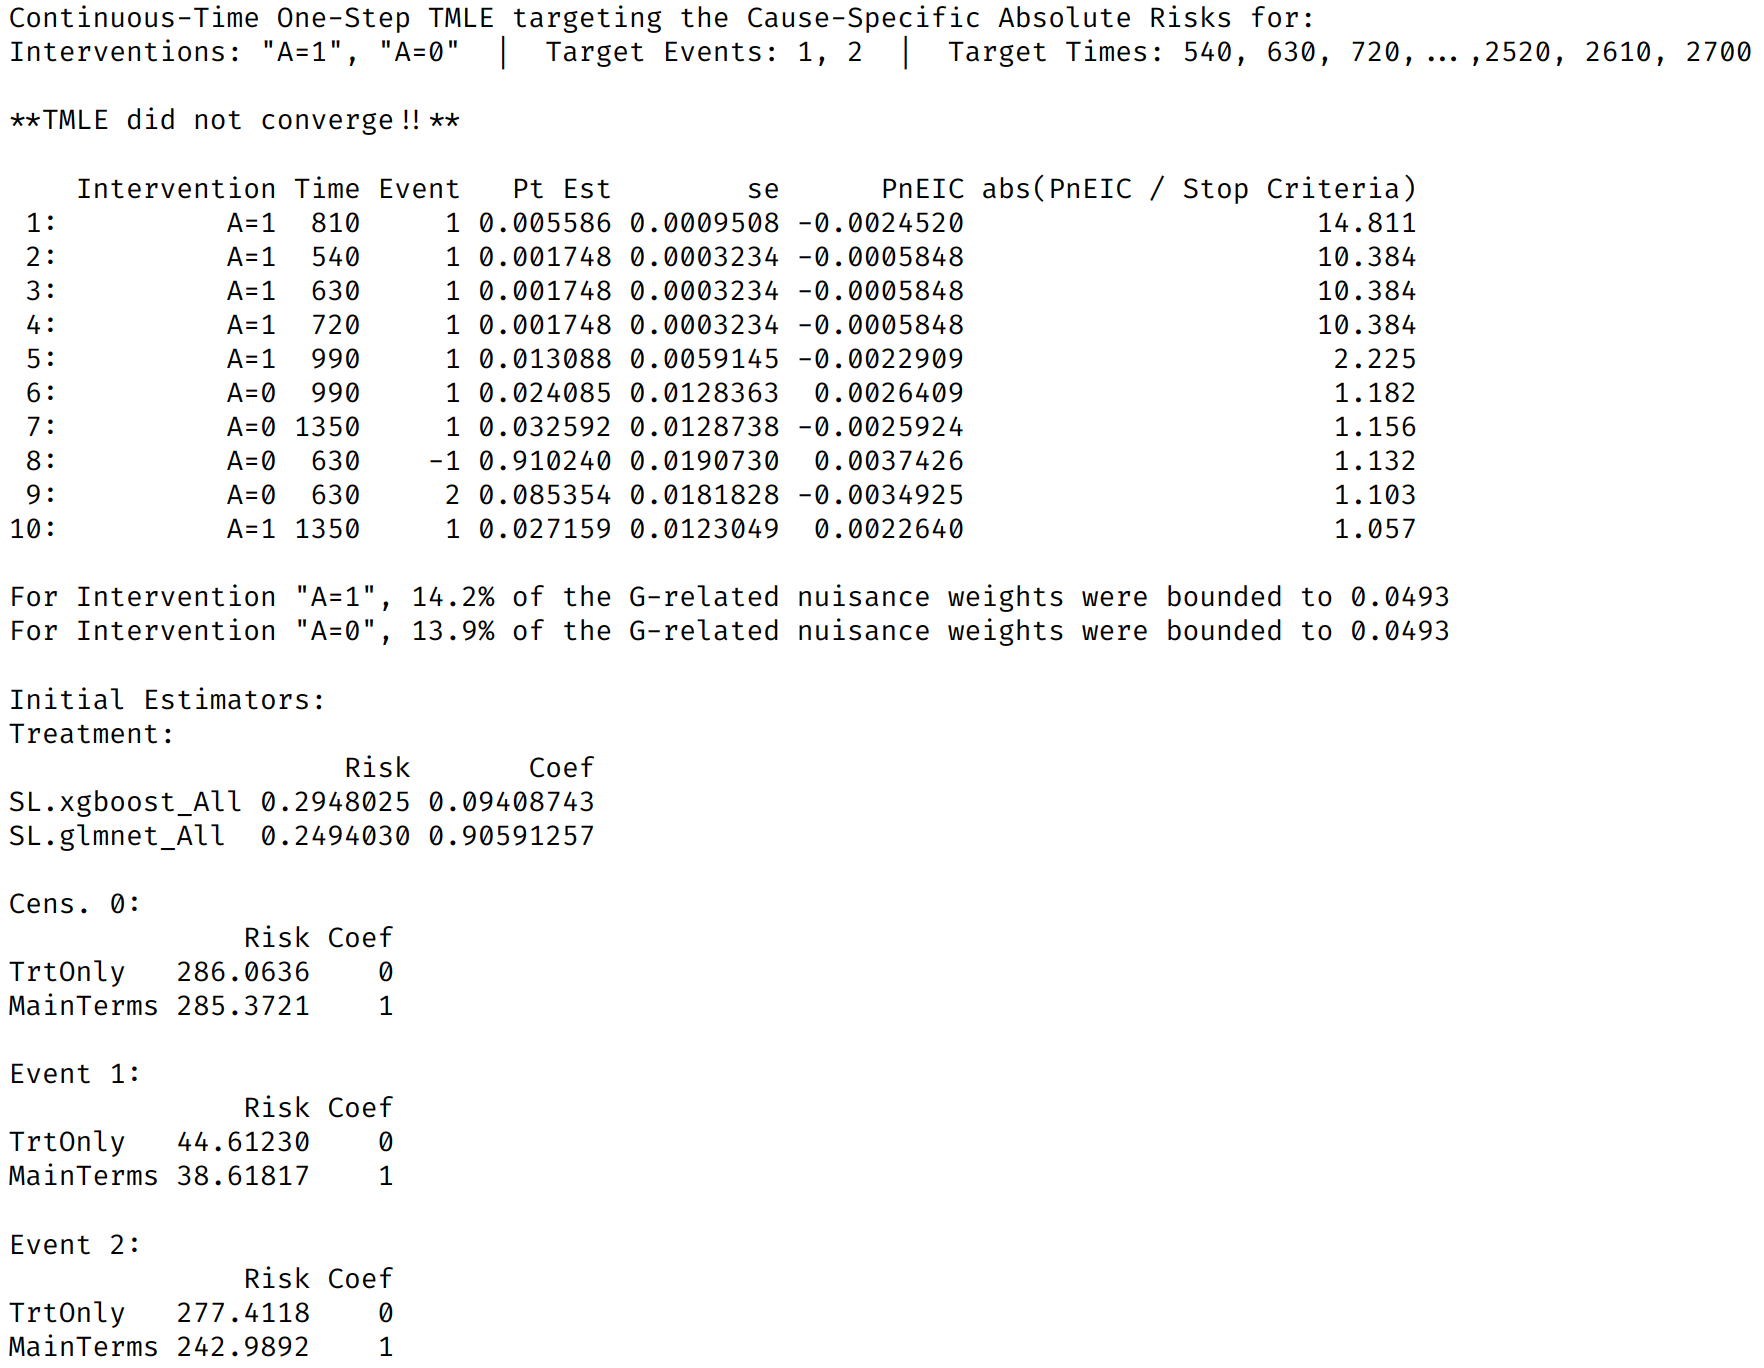
\includegraphics[width=\linewidth]{fig/ConcreteEst.png}
\end{figure}

If TMLE has not converged, the mean EICs that have not attained the desired cutoff will be displayed in a table. Convergence can be attained by increasing the maximum number of iterations, though as seen above, even very small PnEIC values may not meet the convergence criteria at target times when very few events have yet occurred.

The amount of g-related nuisance parameter truncation for each intervention is also printed, and if users suspect positivity issues, the plot method for \code{"ConcreteEst"} objects can be used to visualize the distribution of estimated propensity scores for each intervention, with the red vertical line marking the cutoff for truncation. 

\lstset{language=r,label= ,caption= ,captionpos=b,numbers=none,otherkeywords={}, deletekeywords={}}
\begin{lstlisting}
plot(ConcreteEst, propscores = TRUE)
\end{lstlisting}

\begin{figure}[H]
\center
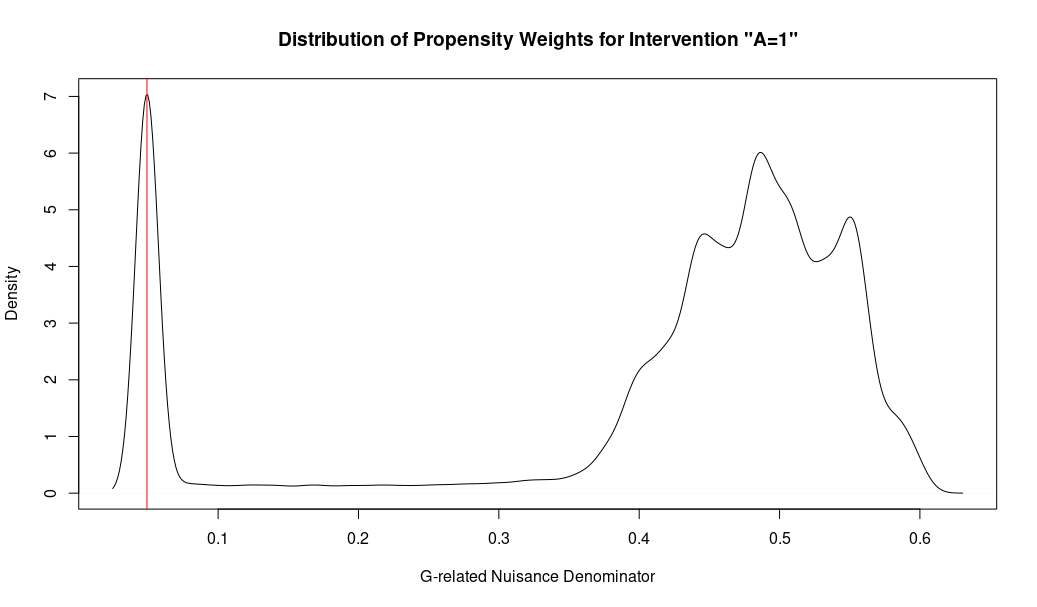
\includegraphics[width=\linewidth]{fig/A1-propscores.png}
\end{figure}

Propensity scores close to 0 indicate the possibility of positivity violations and may warrant re-examining the target time(s), interventions, and covariate adjustment sets. In typical survival applications, positivity issues may arise when targeting times at which some subjects are highly likely to have been censored, or if certain subjects are unlikely to have received a desired treatment intervention.

\subsection{getOutput()}
\label{getoutput}
\code{getOutput()} takes as an argument the \code{"ConcreteEst"} object returned by \code{doConcrete()} and returns tables and produces plots of the cause-specific risks, risk differences, and/or relative risks. By default \code{getOutput()} returns a data.table with point estimates and pointwise standard errors for cause-specific absolute risks, risk differences, and risk ratios. Risk difference and ratios are by default computed by subtracting or dividing the second listed intervention from the first. Below we show a subset of the relative risk estimates produced by the "nutshell" estimation specification for the pbc dataset. 

\lstset{language=r,label= ,caption= ,captionpos=b,numbers=none,otherkeywords={}, deletekeywords={}}
\begin{lstlisting}
getOutput(ConcreteEst, "RR", GComp = FALSE)
\end{lstlisting}

\begin{figure}[H]
\centering
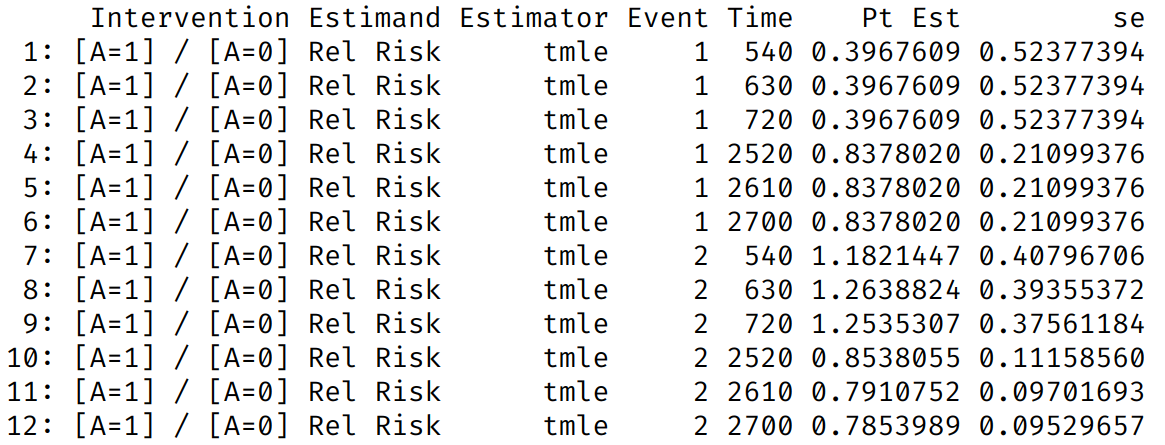
\includegraphics[width=.7\linewidth]{fig/rr-tbl.png}
\end{figure}

From this small sample risk ratios we can see that the treatment decreases the incidence of transplant (event 1) and leads to an increased incidence of death (event 2) earlier on followed by a decreased risk of death. We also see that these treatment effect estimates do not reach a 95\% level of significance. The full table is not shown here because it would take too much space, as can often be the case when estimands involve many time points. Instead results may be more easily interpreted when plotted, as we do below with the treated and control cause-specific risks for transplant and death.

\begin{figure}[H]
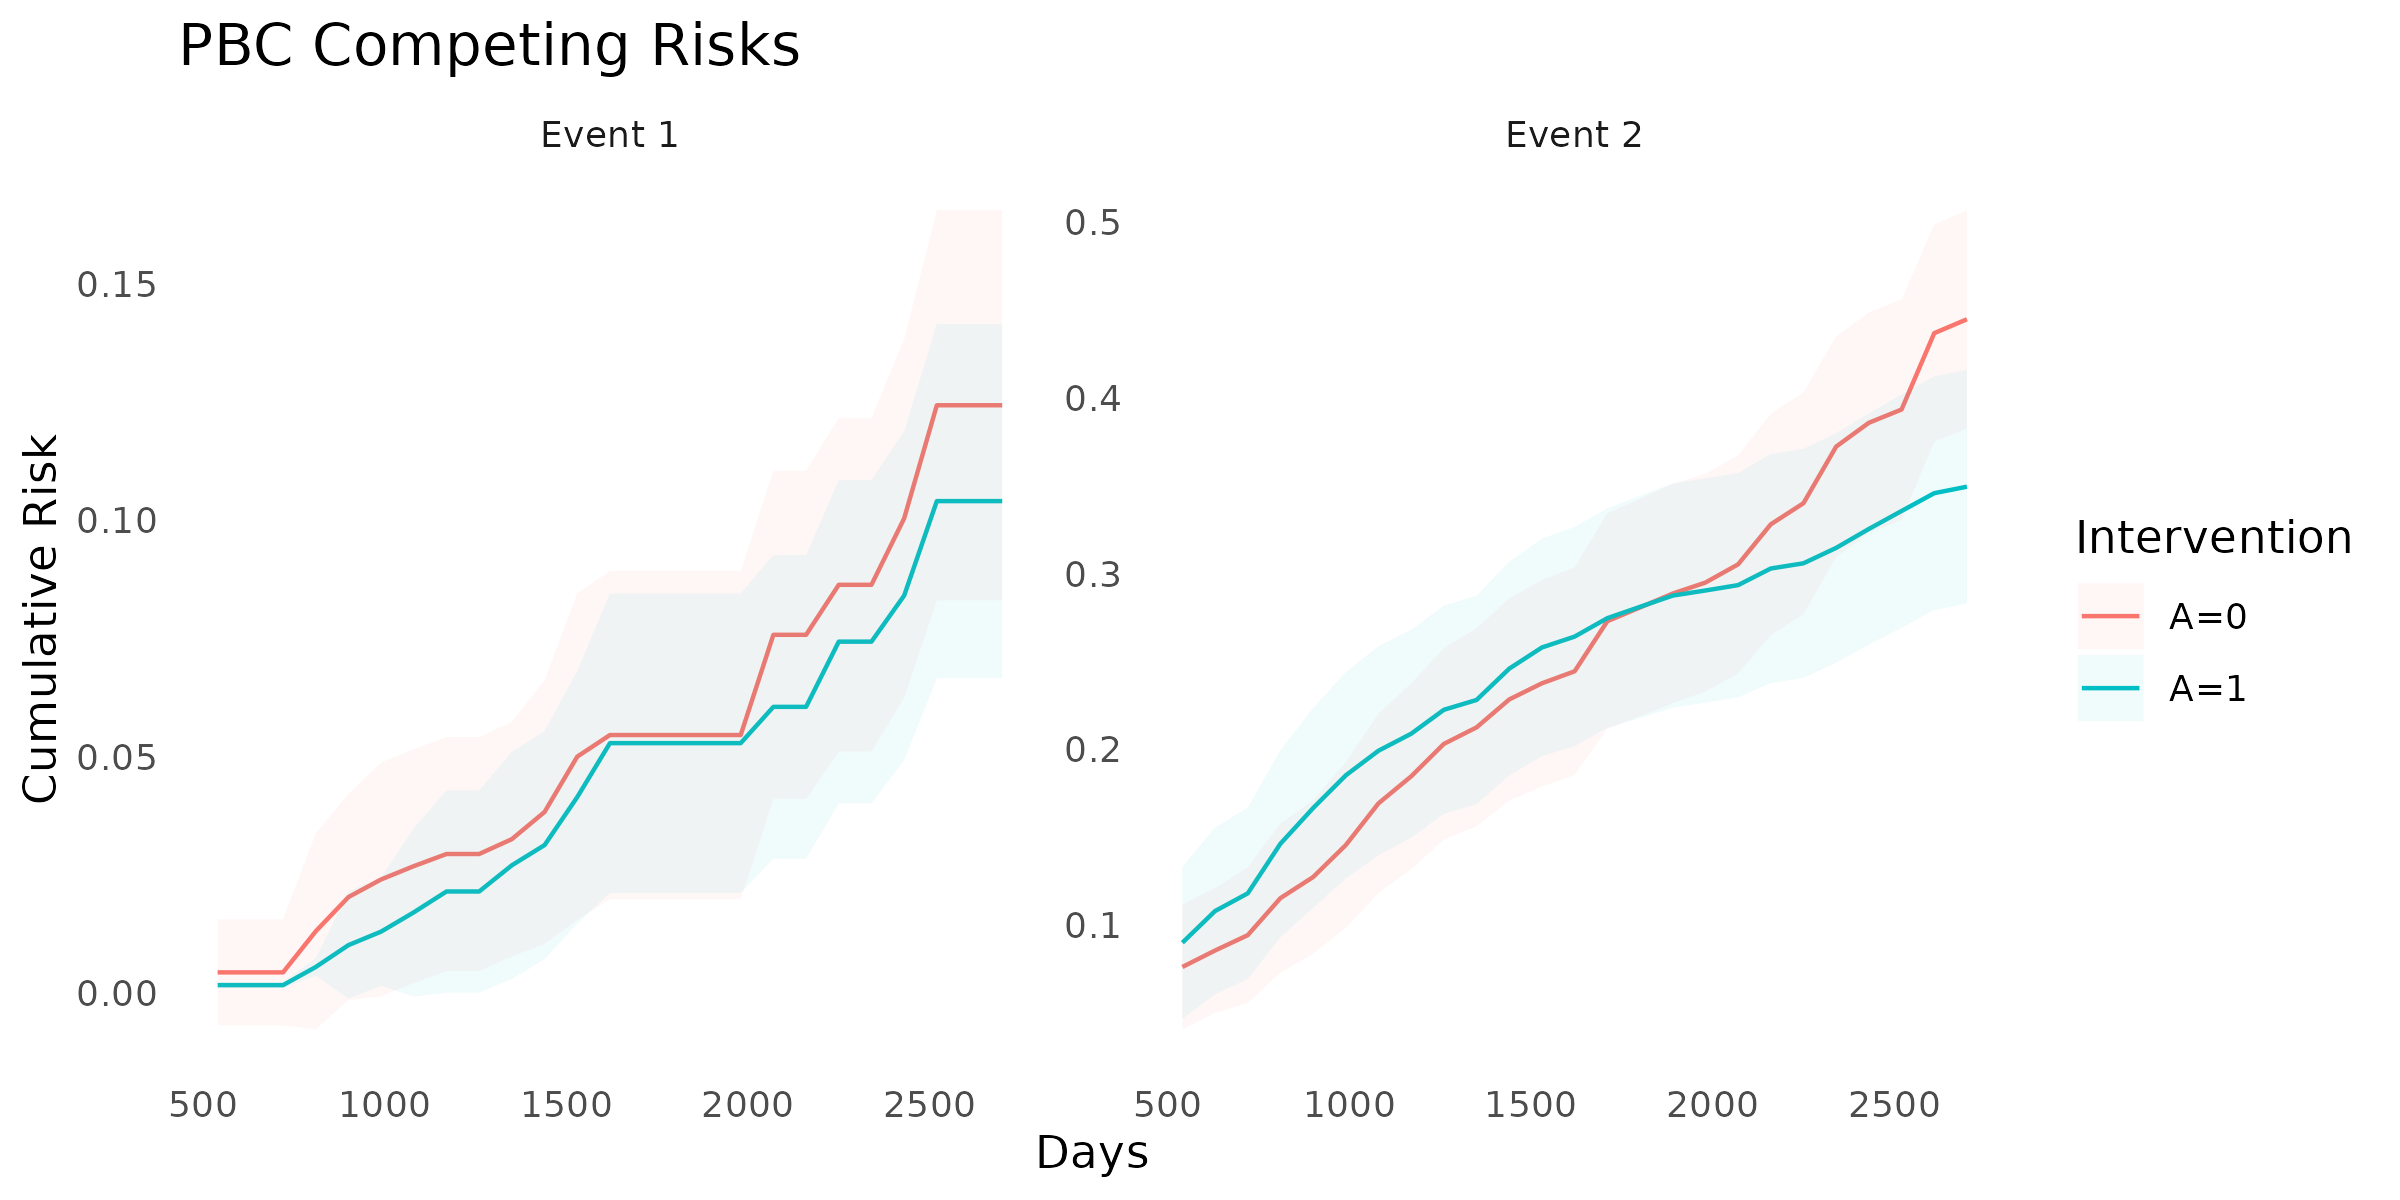
\includegraphics[width=\linewidth]{fig/concrete-pbc.png}
\end{figure}

Here, by comparing the treated and control cumulative incidence curves we can more clearly see the effect of treatment on incidence of both transplant and death, and especially how the treatment effect on risk of death varies over time. 

\section{Diagnostics and Debugging}
\label{sec:org5e6ce4d}

\subsection{Nuisance Weight Truncation Simulation}
\label{sec:org4ce6654}


\section{Appendix: Nice to have Concepts}
\label{sec:org38c2dc8}

\subsection{Identification}
\label{identification}
In order to identify causal estimands such as absolute risk ratios and differences with functions of the observed data, some untestable structural assumptions must hold - namely the assumptions of consistency, positivity, randomization, and coarsening at random on the conditional density of the censoring mechanism. 


\begin{enumerate}
\item The consistency assumption states that the observed outcome given a certain treatment decision is equal to the corresponding counterfactual outcome
\end{enumerate}
\[ T^d_j = T_j \text{ on the event that A = d(L)} \]

\begin{enumerate}
\item The positivity assumption states that the desired treatment regimes occur with non-zero probability in all observed covariate strata, and that remaining uncensored occurs with non-zero probability in all observed covariate strata at all times of interest \(t\).
\end{enumerate}
\[ P_0\left( A = d(L) \mid \L \right) > 0 \;,\, a.e. \]
\[ P(C \geq t \mid a, \L) \;,\, a.e. \]

\begin{enumerate}
\item The randomization assumption states that there is no unmeasured confounding between treatment and counterfactual outcomes
\end{enumerate}
\[ A \indep (T^d_1, T^d_2) \mid \L \]

\begin{enumerate}
\item Coarsening at random on censoring
\end{enumerate}
\[ C \indep (T^d_1, T^d_2) \mid T > C, A, \L \]

Given coarsening at random, the observed data distribution factorizes 
\begin{align*}
p_0(O) = p_{0}(\L)\, \g_0(A \mid \L)\, \lambda_{0,c}&(\T \AX)^{\1(\Delta = 0)} S_{0, c}(\T\text{-} \AX)\\
&\prod_{j=1}^{J} S_{0}(\T\text{-} \AX) \, \lambda_{0,j}(\T \AX)^{\1(\Delta = j)}
\end{align*}
where \(\lambda_{0,c}(t \AX)\) is the true cause-specific hazard of the censoring process and \(\lambda_{0,j}(t \AX)\) is the true cause-specific hazard of the \(j^{th}\) event process. Additionally
\begin{align*}
    S_{0,c}(t \ax) &= \exp\left(-\int_{0}^{t} \lambda_{0,c}(s \ax) \,ds\right)
\intertext{while in a pure competing risks setting}
    S_0(t \ax) &= \exp\left(-\int_{0}^{t} \sum_{j=1}^{J} \lambda_{0,j}(s \ax) \,ds\right)
\intertext{and} 
    F_{0,j}(t \ax) &= \int_{0}^{t} S(s\text{-} \ax) \lambda_{0,j}(s \ax)\,ds\\
    &= \int_{0}^{t} \exp\bigg(-\int_{0}^{s} \sum_{j=1}^{J} \lambda_{0,j}(u \ax)\,du\bigg) \lambda_{0,j}(s \ax)\,ds.
\end{align*}

Under the above identification assumptions, the post-intervention distribution of \(O\) under intervention \(A=d(a, \l)\) in the world of no-censoring, i.e the distribution of \((\L,\, T^d_j,\, \Delta^d_j :\, j = 1, \dots, J)\), can be represented by the so-called G-computation formula. Let’s denote this post-intervention probability distribution with \(P_{d}\) and the corresponding post-intervention random variable with \(O_d\). The probability density of \(O_d\) follows from replacing \(\g_0(A \mid \L)\) with the density that results from setting \(A = d(a, l)\), \(\g_d(d(A, \l) \mid \L)\), and replacing the conditional probability of being censored at time \(t\) by no censoring with probability \(1\). In notation, \(P(O_d = o)\) is given by
\begin{align*}
p_{d}(o) = p_{0}(\l) \, &\g_d(d(a, \l) \mid \l) \, \1(\delta \neq 0)\\
&\prod_{j=1}^{J} \left[S_{0}(\t\text{-} \mid A = d(a, \l),\, \l) \, \lambda_{0,j}(\t \mid A = d(a, \l), \l)^{\1(\delta = j)} \right]
\end{align*}
Recalling the censoring and cause-specific conditional hazards defined above in terms of observed data, we should note that given the identifiability assumptions they now identify their counterfactual counterparts, i.e. 
\[\lambda_{c}(t \mid W,\, A) = \lim_{h \to 0}P(C < t + h \mid C \geq t,\, W,\, A)\]
\[\lambda_{j}(t \mid W,\, A)= \lim_{h \to 0}P(T < t+h, J=j \mid T \geq t, W, A)\]
Note that the cause-specific event hazards are not conditional on censoring once identifiability assumptions are met.

Since the density \(P(O_d=o)\) implies any probability event about \(O_d\), this g-computation formula for \(P(O_d=o)\) also implies g-computation formulas for causal quantities such as event-free survival and cause-\(k\) absolute risk under intervention \(d\). 

\newpage
\bibliography{main.bib}
\end{document}